\documentclass[11pt]{beamer}
\usetheme{JuanLesPins}
\usepackage[utf8]{inputenc}
\usepackage{amsmath}
\usepackage{amsfonts}
\usepackage{amssymb}
\usepackage{graphicx}
\usepackage{subfig}
\usepackage{listings}
\author{Grupo de Propagação - GAPTEM}
\title{Proposta de Padronização Para Entrada e Saída de Dados}
%\setbeamercovered{transparent} 
%\setbeamertemplate{navigation symbols}{} 
%\logo{} 
%\institute{} 
%\date{} 
%\subject{} 
\begin{document}

\begin{frame}
\titlepage
\end{frame}

\begin{frame}
	\frametitle {Objeto}
Definir uma padronização a ser utilizada no Grupo de Propagação do GAPTEM, que permita o intercâmbio de informações entre os diversos \textit{solvers} que venham a ser desenvolvidos dentro do grupo.\\
Devendo contemplar:
	\begin{itemize}
		\item Configuração da simulação
		\item Entrada de dados
		\item Resultados da simulação
	\end{itemize}
*\emph{Propõem-se que todas as variáves sejam apresentadas utilizando a utidade padronizada pelo S.I., no formato inteiro ou ponto flutuante}
\end{frame}

\begin{frame}
\frametitle{Configuração da simulação}
Propõe-se a adoção do formato Json pelos seguintes motivos:
	\begin{itemize}
		\item \textbf{JSON} (\textit{JavaScript Object Notation}) é um modelo para armazenamento e transmissão de informações no formato texto.
		\item Permite a criação de forma compacta e estruturada dos parâmetros desejados, preservando o tipo da variável.
		\item Sua leitura é de fácil implementação e bastante difundida em várias linguagens de programação.	
	\end{itemize} 
\end{frame}

\begin{frame}
\frametitle{Importar \textit{.json} no  Matlab \textregistered}
	\begin{itemize}
		\item No Matlab$^{\textregistered}$ um arquivo \textit{.json} pode ser convertido para um objeto do tipo 						\textit{struct}
		\item Os arquivos \textit{.json} são importados através do comando:\\ \textit{var\_x $=$ jsondecode$($ fileread $($ 'file\_name.json' $) )$}
	\end{itemize}
\end{frame}

\begin{frame}
\frametitle{Importar \textit{.json} no  Matlab\textregistered} 
Exemplo: conf\_teste.json
	\begin{figure}
			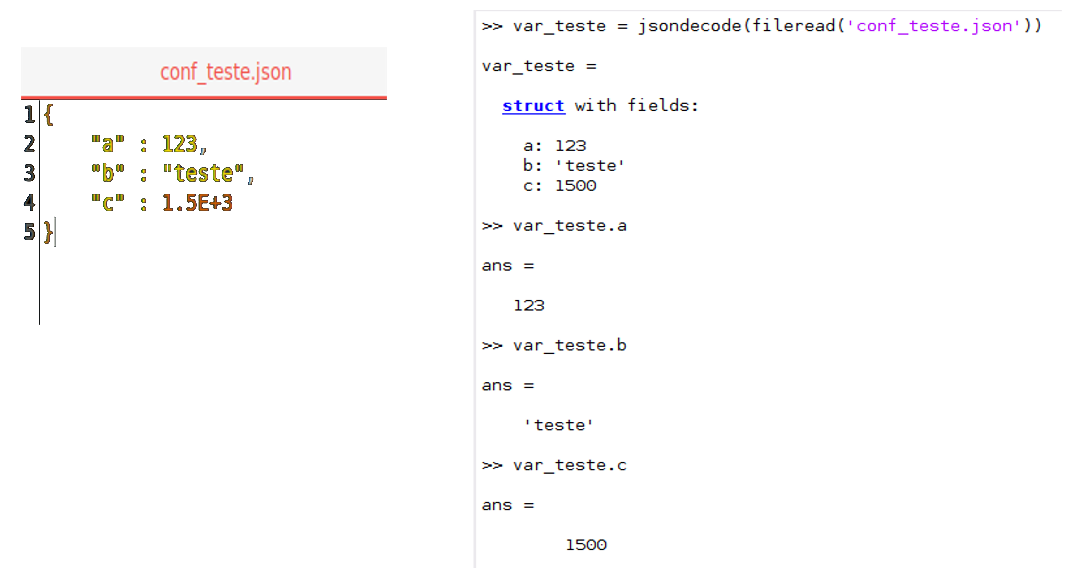
\includegraphics[scale=0.3]{ler_json_matlab}
	\end{figure}
\end{frame}

\begin{frame}[fragile]
	\frametitle{Importar \textit{.json} em  Python}
	\begin{itemize}
		\item Em Python um arquivo \textit{.json} pode ser convertido para um objeto do tipo \textit{dictionary}.
		\item A estrutura dos arquivos \textit{.json} é compreendida utilizando a biblioteca ''json'':
	\end{itemize}
\begin{lstlisting}[language=python]
	import json
	f = 'file_name.json'
	with open(f) as json_conf : 
		var_x = json.load(f)
\end{lstlisting}

\end{frame}

\begin{frame}
	\frametitle{Importar \textit{.json} em Python} 
	Exemplo: conf\_teste.json
	\begin{figure}
		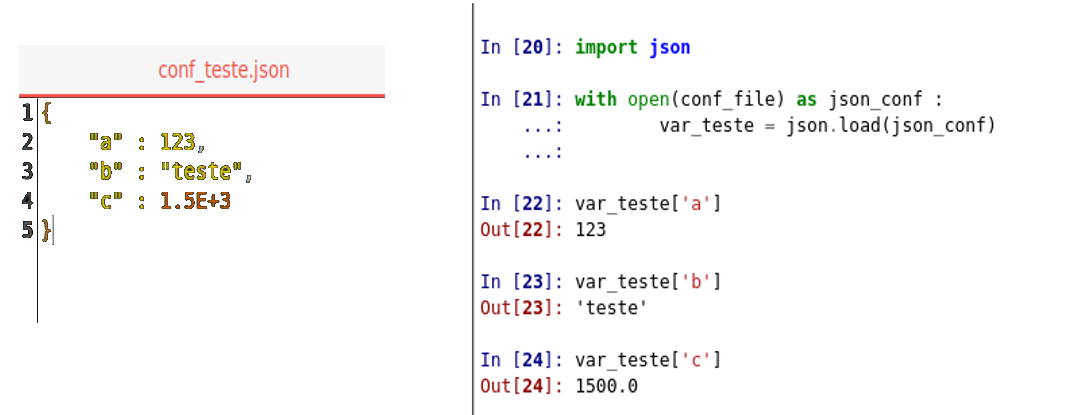
\includegraphics[scale=0.3]{ler_json_python}
	\end{figure}
\end{frame}

\begin{frame}
	\frametitle{Arquivo de configuração}
	\begin{itemize}
		\item Propõe-se que o nome do arquivo seja:\\
		\textit{conf\_}\textbf{\{frequencia central\}}\textit{.json}\\
		p.ex: conf\_400MHz.json, conf\_15GHz.json
		\item As informações dos parâmetros de simulação sejam apresentados em blocos.
	\end{itemize}
\end{frame}

\begin{frame}
	\frametitle{Estrutura do arquivo de configuração}
	\centering
	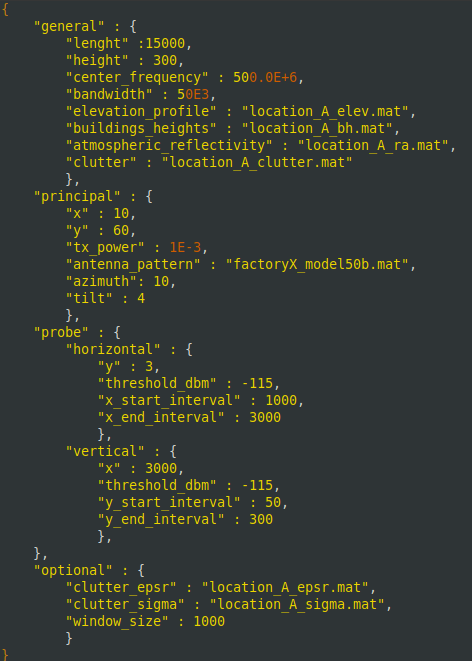
\includegraphics[scale=0.3]{json}
\end{frame}

\begin{frame}
	\frametitle{Entrada de Dados}
	São considerados dados as informações descritivas de:
	\begin{itemize}
		\item Elevação do Terreno
		\item Altura das Edificações
		\item Tipo de Cobertura do Terreno
		\item Diagramas de irradiação das antena
		\item Comportamento do Índice de Refratividade da Atmosfera
	\end{itemize}
\end{frame}

\begin{frame}
	\frametitle{Entrada de Dados}
	Propõem-se a utilização de \textit{m-files}.\\
	Cada informação em um arquivo distinto contendo:
	\begin{itemize}
		\item Uma matriz $1xN$ contendo a posição relativa da informação
		\item Uma matriz $1xN$ contendo a informação relativa ao ponto de coleta
		\item Uma variável de dados informando o passo utilizado
	\end{itemize}
\end{frame}

\begin{frame}
	\frametitle{Dados ao longo do eixo X}
	Para as informações ao longo do eixo X, p.ex. elevação, clutter, altura de edificações, a referência é a estação principal (p.ex eNB, transmissora de radiodifusão).\\
	O \textit{m-file} deve conter três variáveis: 
	\begin{itemize}
		\item uma matriz $1xN$ contendo as distâncias relativas das amostras tomando a estação principal como referência denominada \emph{distancia}
		\item uma matriz $1xN$ contendo os valores do parâmetro amostrado nos pontos cujas distâncias estão indicadas pelo mesmo índice na matriz \emph{distancia}. O nome desta matriz segue o nome do parâmetro observado em formato \textit{ASCII} (caixa baixa, sem acentos).
		\item O passo utilizado para amostragem.
	\end{itemize}
	Para as informações de classificação de cobertura do terreno, sugere-se adoção dos códigos do \textit{Land Cover Classification System} (LCCS).
\end{frame}

\begin{frame}
	\frametitle{Dados ao longo do eixo X - exemplo}
		\begin{figure}
		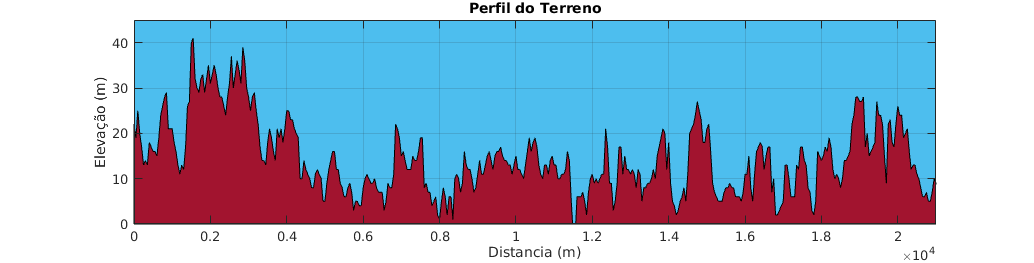
\includegraphics[scale=0.3]{exemplo_elevacao_grafico}
		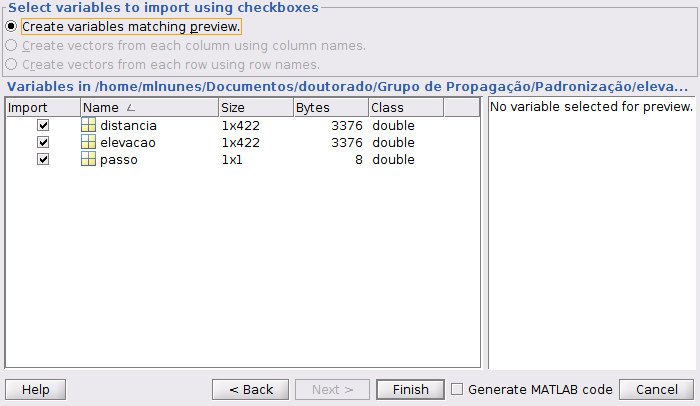
\includegraphics[scale=0.3]{exemplo_elevacao}
	\end{figure}
\end{frame}

\begin{frame}
	\frametitle{Dados ao longo do eixo Y}
	Para as informações ao longo do eixo Y, p.ex. índice de refratividade da atmosfera, a referência é nível do mar.\\
	O \textit{m-file} deve conter três variáveis: 
	\begin{itemize}
		\item uma matriz $1xN$ contendo a faixa de altitude de coleta das amostras, denominada \emph{altitude}
		\item uma matriz $1xN$ contendo os valores do parâmetro amostrado nos pontos cujas altitudes estão indicadas pelo mesmo índice na matriz \emph{altitude}. O nome desta matriz segue o nome do parâmetro observado em formato \textit{ASCII} (caixa baixa, sem acentos).
		\item O passo utilizado para amostragem.
	\end{itemize}

\end{frame}

\begin{frame}
	\frametitle{Diagramas de irradiação de antenas}
	O \textit{m-file} deve conter três variáveis: 
	\begin{itemize}
		\item uma matriz $1xN$ contendo o azimute denominado \textit{azimute}
		\item uma matriz $1xN$ contendo os valores do ganho no plano H amostrados nos pontos cujos azimutes estão indicadas pelo mesmo índice na matriz \emph{azimute}, denominada \textit{plano\_h}.
		\item uma matriz $1xN$ contendo os valores do ganho no plano V amostrados nos pontos cujos azimutes estão indicadas pelo mesmo índice na matriz \emph{azimute}, denominada \textit{plano\_v}.
		\item O passo utilizado para amostragem.
	\end{itemize}
	
\end{frame}

\begin{frame}
	\frametitle{Saída de dados}
		Propõe-se que os dados de saída sejam disponibilizados em formato \emph{M-file} contendo na descrição a variável amostrada e a grandeza utilizada. 
\end{frame}

\begin{frame}
	\centering
	{\Huge Aguardo sugestões.}
	\parbox{\linewidth}{\vspace*{30pt}\centering mlnunes@ufmg.br}
	
	\footnotesize\parbox{\linewidth}{\vspace*{90pt}O arquivo fonte desta apresentação em formato {\LaTeX} está disponível em \url{https://github.com/mlnunes/padronizacao_grupo_propagacao.git}.}
\end{frame}

\end{document}